% Layout for fig11: 2x2 block on the left, panel (e) full height on the right.
%
% All five panels came from one figure, so a SINGLE scale factor reproduces the
% original geometry.  The fractions below are each panel's natural width divided
% by the assembled natural width (1486.3 pt = 524.3 mm), with 2 mm gaps:
%
%   fig11a 392.61 x 388.86 pt      fig11c 441.09 x 433.98 pt
%   fig11b 467.48 x 388.86 pt      fig11d 466.04 x 433.98 pt
%   fig11e 567.80 x 800.76 pt
%
% a/b share a height and c/d share a height, so each row aligns automatically.
% The top row is naturally narrower than the bottom one (as in the original),
% so it is centred rather than stretched -- use \hspace, not \hfill.
%
% Needs a wide text block: figure* in two-column, or \usepackage{rotating}
% and sidewaysfigure in one-column.

\begin{figure}[t]
  \centering
  % ---- left: the 2x2 block -------------------------------------------
  \begin{minipage}[c]{0.6142\linewidth}
    \centering
    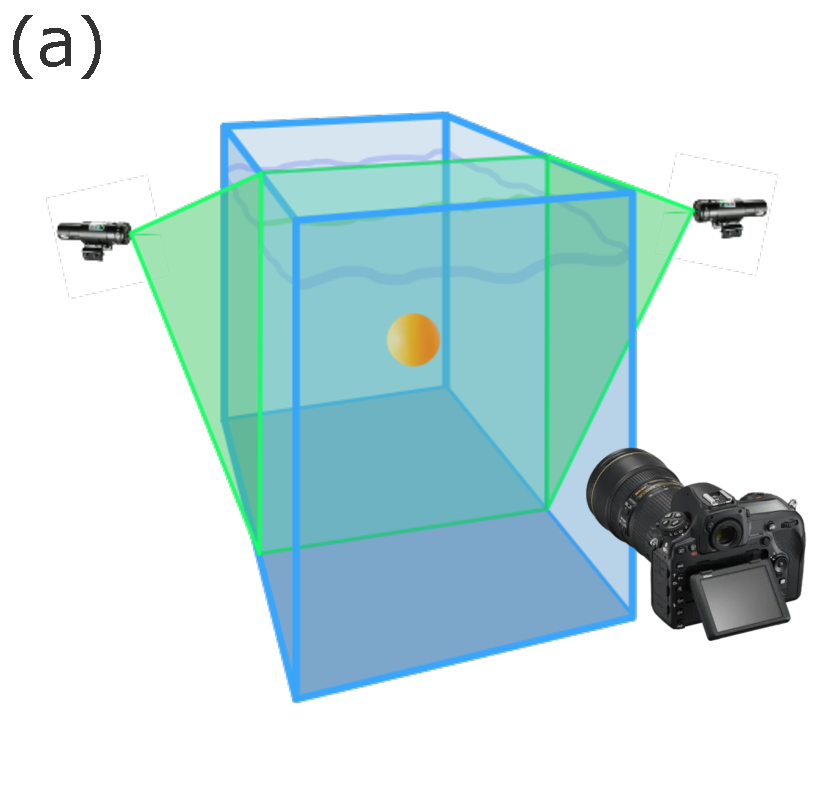
\includegraphics[width=0.4301\linewidth]{fig11a}%
    \hspace{0.0062\linewidth}%
    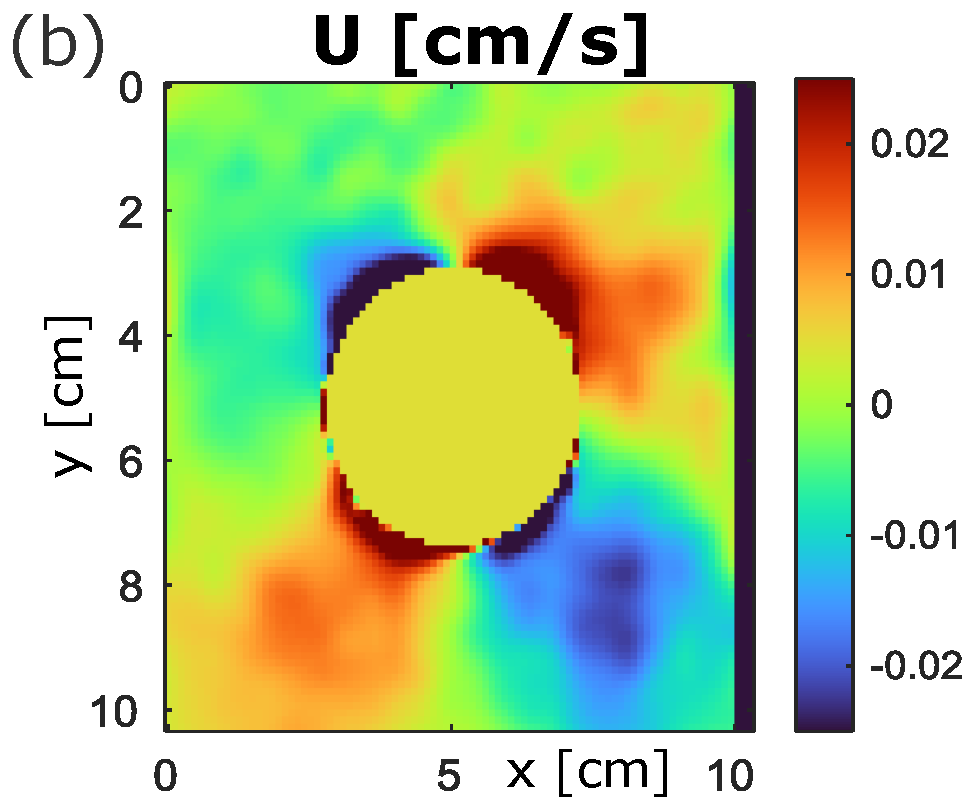
\includegraphics[width=0.5121\linewidth]{fig11b}\\[1.5mm]
    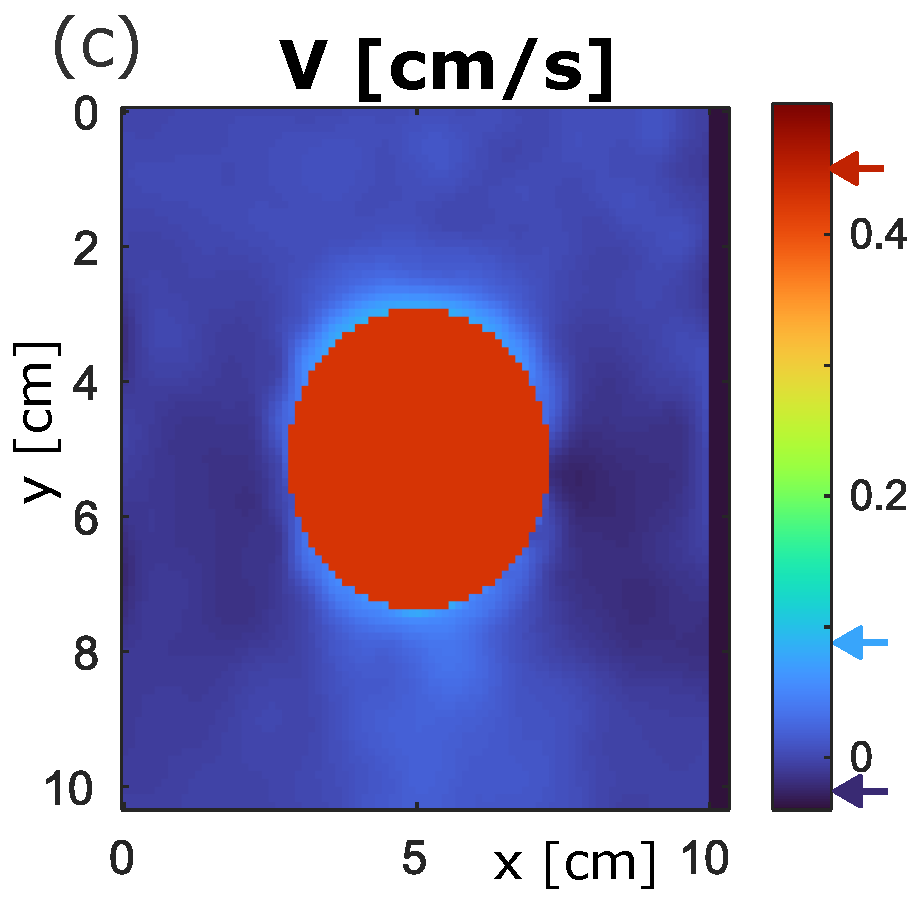
\includegraphics[width=0.4832\linewidth]{fig11c}%
    \hspace{0.0062\linewidth}%
    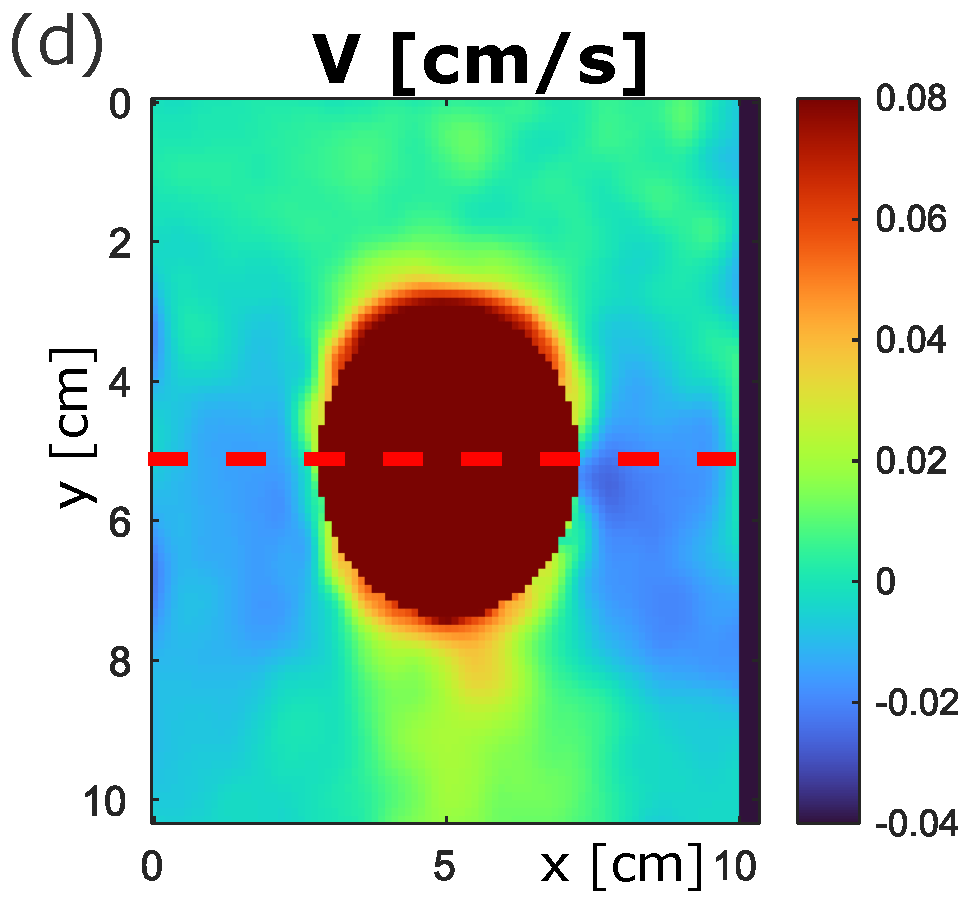
\includegraphics[width=0.5106\linewidth]{fig11d}
  \end{minipage}%
  \hspace{0.0038\linewidth}%
  % ---- right: panel (e), spanning both rows ---------------------------
  \begin{minipage}[c]{0.3820\linewidth}
    \centering
    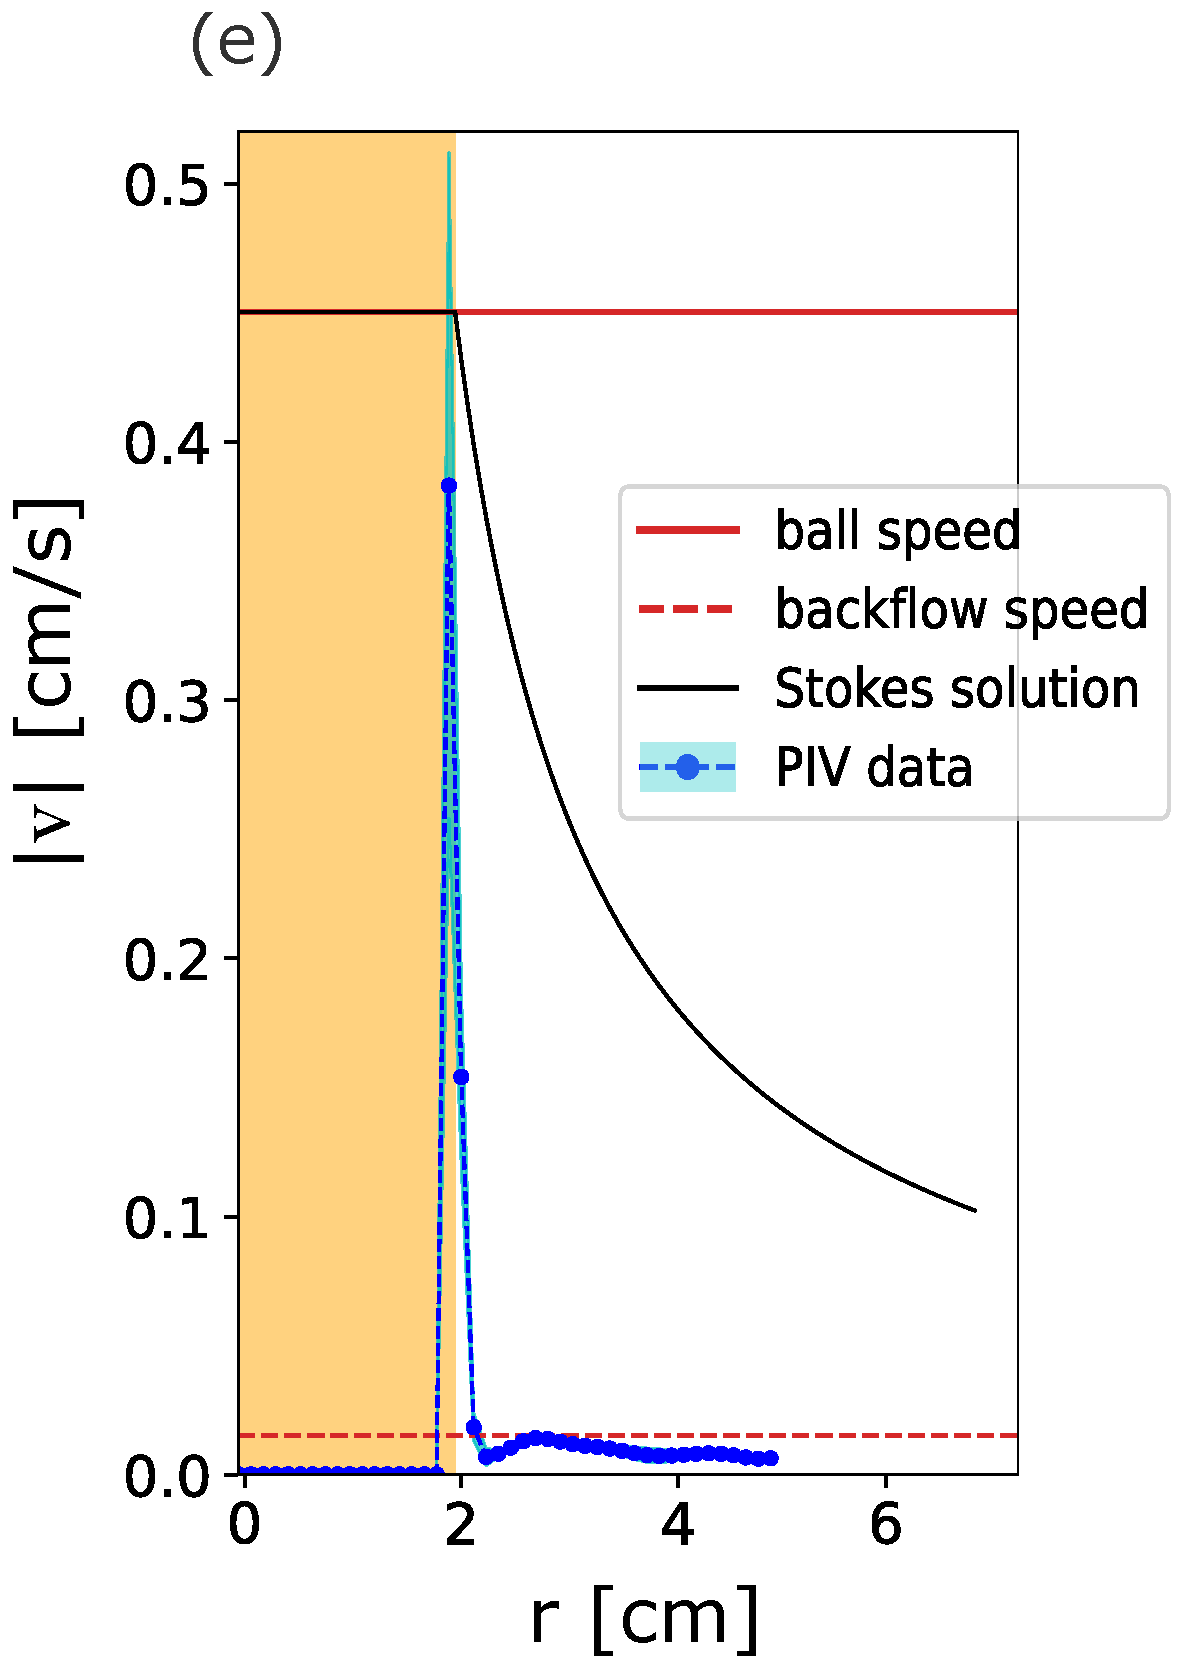
\includegraphics[width=\linewidth]{fig11e}
  \end{minipage}
  \caption{...}
  \label{fig:piv}
\end{figure}
